\section{\method: Dual-Layer Interpretable Accident Anticipation}
\label{sec:method}

We present \method{}, a unified framework for intrinsically interpretable
accident anticipation. Figure~\ref{fig:framework} gives an overview.
We describe each component in order of information flow.

\begin{figure*}[t]
  \centering
  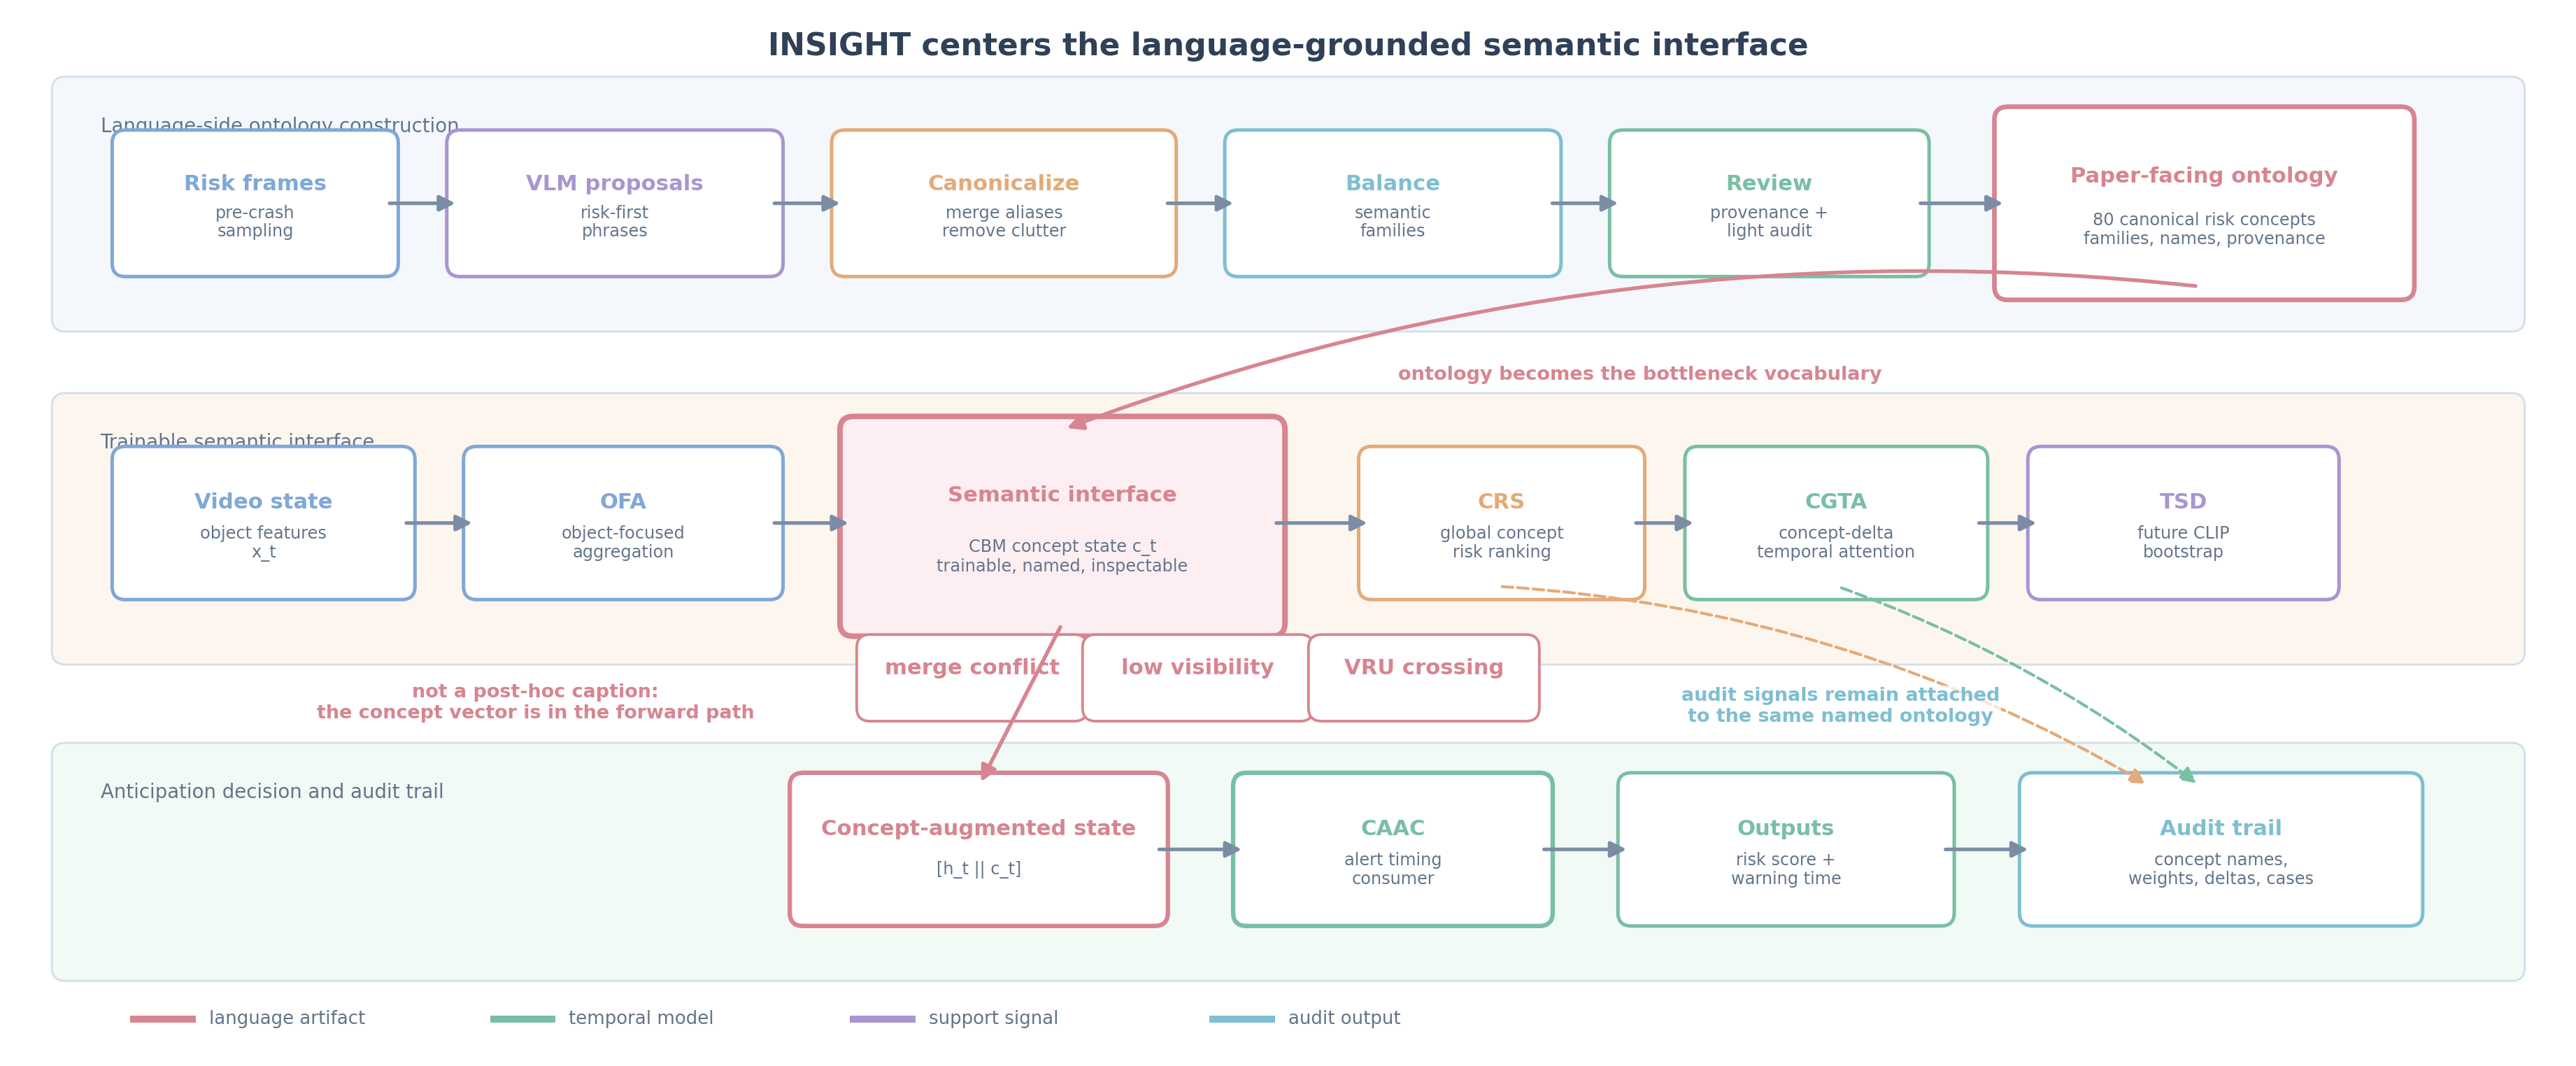
\includegraphics[width=\textwidth]{../figures/insight_framework.pdf}
  \caption{\textbf{INSIGHT framework overview.} Per-frame information flows
  left-to-right through five modules. The \textcolor{red}{\textbf{WHY layer}}
  (CBM) maps object features to $K{=}837$ interpretable risk concepts
  $\mathbf{c}_t$. The \textcolor{green!50!black}{\textbf{WHEN layer}}
  (CAAC) uses concept-augmented state $\mathbf{s}_t=[\mathbf{h}_t\|\mathbf{c}_t]$
  to optimise alert timing via a time-remaining reward. CRS provides an
  auditable per-concept risk ranking; CGTA links temporal attention to
  concept dynamics; TSD distils CLIP future features for anticipatory
  representations. The dashed arc (CBM$\to$CAAC) denotes the concept
  state pathway that makes every alert decision concept-traceable by construction.}
  \label{fig:framework}
\end{figure*}

\subsection{Problem Formulation}

Given a dashcam video $\{\mathbf{x}_t\}_{t=1}^T$ with
$\mathbf{x}_t \in \mathbb{R}^{N \times D}$
($N{=}19$ detected objects, $D{=}4096$ VGG16~\citep{ref31} ROI features),
a binary label $y \in \{0,1\}$, and time-of-accident $\tau$,
\method{} is motivated by the following idealised objective:
\begin{equation}
  \max_{\theta}\; \mathbb{E}[\mathrm{TTA}]
  \quad \text{s.t.} \quad \mathrm{AP}(\theta) \geq \mathrm{AP}_{\text{base}},
  \label{eq:objective}
\end{equation}
where $\mathrm{TTA} = (\tau - t^*)/\mathrm{fps}$ and
$t^* = \min\{t : \pi_\theta(\mathrm{alert}\mid\mathbf{s}_t) \geq 0.5\}$
is the first alert frame.
This objective should be read as a \emph{motivational target} rather than as
a literal constrained solver used in optimization. In practice, we implement a
surrogate multi-loss training objective that balances classification,
concept supervision, timing control, and anticipatory representation learning,
and we evaluate the resulting AP--mTTA trade-off empirically.

\subsection{Overview}

\paragraph{Design intuition.}
The central design principle of \method{} is simple:
\emph{concepts should not merely explain the prediction after the fact;
they should participate directly in the decision process itself}.
To achieve this, \method{} first extracts an interpretable concept state,
then uses those concepts to modulate temporal attention, risk scoring,
and finally the Actor-Critic timing policy.
This tight coupling between semantics and sequential decision-making
is what enables simultaneous WHY and WHEN transparency.

The per-frame forward pass is:
\begin{align*}
  \mathbf{x}_t
  &\xrightarrow{\text{OFA}} \mathbf{o}_t
  \xrightarrow{\cbm} (\mathbf{c}_t,\mathbf{e}_t)
  \xrightarrow{\crs} \rho_t \\
  &\xrightarrow{\cgta} \mathbf{g}_t
  \xrightarrow{\text{GRU}} \mathbf{h}_t
  \xrightarrow{\caac} (p_t, a_t, V_t).
\end{align*}
The key design choice is that the \caac{} MDP state
$\mathbf{s}_t = [\mathbf{h}_t \| \mathbf{c}_t]$ explicitly includes
concept activations, making every alert-timing decision concept-traceable
by construction.

\subsection{Object-Focused Aggregation}

The $N$ object features per frame are aggregated by an Object-Focused
Attention (OFA) module:
\begin{align}
  \alpha^n_t &= \mathrm{softmax}_n\bigl(\mathbf{w}_a^\top
    \tanh(\mathbf{W}_o \mathbf{x}^n_t)\bigr), \\
  \mathbf{o}_t &= \sum_{n=1}^N \alpha^n_t\,\mathbf{W}_f \mathbf{x}^n_t
    \in \mathbb{R}^h.
\end{align}

\subsection{Concept Ontology Discovery and Adjudication}

\paragraph{Why ontology construction matters.}
A concept bottleneck is only as good as its vocabulary.
In accident anticipation, a generic traffic word list is often too broad,
while a fully manual ontology is difficult to scale and easy to bias toward
researcher priors. We therefore treat concept construction itself as part of
our method rather than as an external preprocessing detail. The goal is not to
generate visually descriptive tags, but to produce \emph{trainable,
auditable, and intervention-ready risk primitives} that can serve as the
semantic interface for the WHY layer.

\paragraph{Stage 1: frame mining.}
We first build a frame manifest from positive accident videos by sampling
pre-crash frames that exhibit diverse traffic geometries, actor interactions,
and visibility conditions. This step avoids querying a multimodal model on all
video frames while still covering the semantic support of accident precursors.
Importantly, the sampling policy is risk-oriented: frames are chosen to expose
emerging hazards rather than merely static scene diversity.

\paragraph{Stage 2: multimodal risk concept discovery.}
Given sampled frames, a multimodal language model proposes candidate concepts,
risk factors, and coarse semantic families. Our prompts explicitly ask for
\emph{risk-first} concepts---such as cut-in behaviour, brake-light onset,
visibility degradation, or closing distance---rather than generic scene
captions. The raw output is therefore a noisy but high-recall pool of accident
precursor phrases rather than a polished ontology.

\paragraph{Stage 3: risk-first refinement.}
We then refine the raw pool by prioritising causal or precursor-like factors,
filtering obvious background clutter, merging near-duplicates, and normalising
phrasing toward concise risk primitives. This stage is intentionally asymmetric:
it prefers under-specification over over-fragmentation, because downstream
training benefits more from stable and reusable primitives than from dozens of
near-synonymous micro-concepts.

\paragraph{Stage 4: ontology polishing, family balancing, and human review.}
The final step is no longer just canonical renaming. Starting from the large-vocabulary
academic pool, we perform a dedicated polishing pass that audits family coverage,
consolidates high-priority duplicate clusters (especially visibility, pedestrian-crossing,
and merge-related concepts), normalises naming into short canonical risk phrases,
and then applies a very-light human review over every retained concept.
This transforms the ontology from a high-recall phrase pool into a
\emph{paper-ready semantic interface}: compact enough to present clearly,
rich enough to preserve major accident precursor families, and explicit enough to
support intervention analysis, family-level auditing, and appendix-level ontology reporting.
Figure~\ref{fig:concept_pipeline} visualises the end-to-end process, and
Figures~\ref{fig:concept_evolution} and~\ref{fig:concept_case_study} show how
noisy phrase sets are converted into canonical trainable concepts.

\begin{figure*}[t]
  \centering
  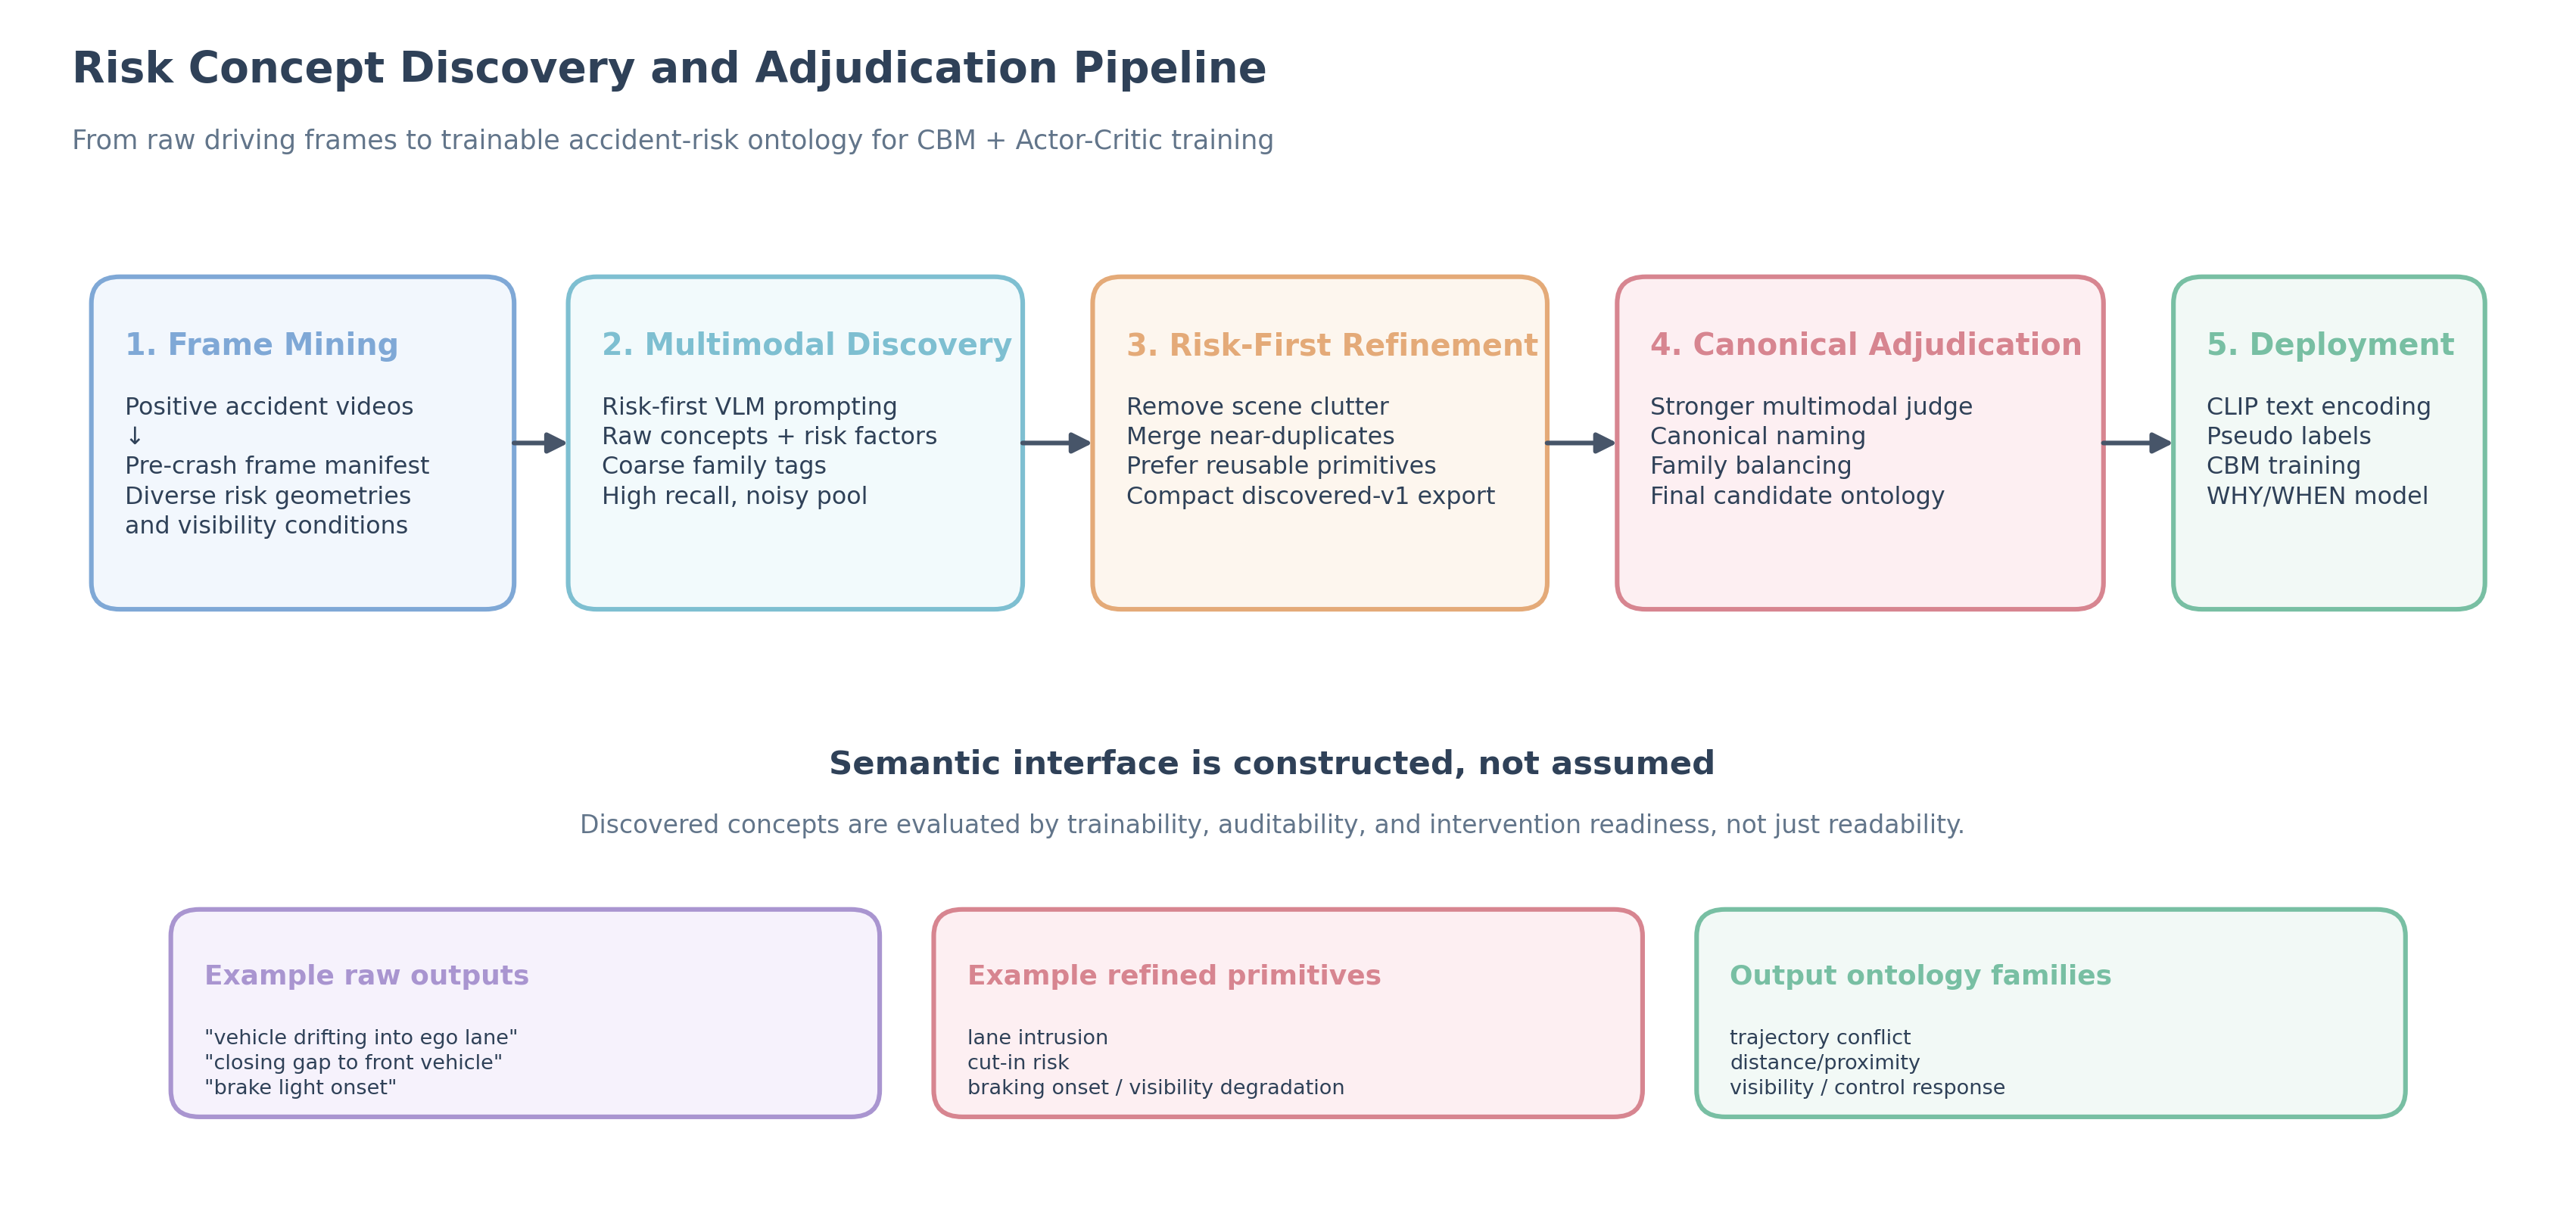
\includegraphics[width=0.98\textwidth]{../figures/insight_fig_concept_pipeline.pdf}
  \caption{\textbf{End-to-end concept ontology construction pipeline.}
  Starting from sampled pre-crash driving frames, the pipeline performs
  multimodal risk-concept discovery, risk-first refinement, duplicate-cluster
  consolidation, family balancing, and light human review to produce a final
  trainable ontology for the concept bottleneck. This figure clarifies that the
  ontology is a reproducible methodological component rather than a hidden fixed
  vocabulary assumption.}
  \label{fig:concept_pipeline}
\end{figure*}

\paragraph{What the final ontology is designed to optimise.}
The final discovered ontology is not selected only for lexical cleanliness.
It is designed to jointly optimise four properties: (i)~semantic plausibility,
(ii)~family coverage, (iii)~trainability in the downstream CBM+Actor--Critic
pipeline, and (iv)~paper-level auditability. This design choice matters.
A compact ontology that is easy to read but too narrow to train well is not
useful; conversely, a broad ontology that trains well but remains lexically noisy
is difficult to defend as a scientific semantic interface.
Our polishing stage therefore treats ontology construction as a structured model-design
problem rather than a cosmetic prompt-engineering step.

\paragraph{Deployment into the CBM.}
The output of the pipeline is a text ontology that can be encoded with CLIP and
used immediately for pseudo concept supervision and concept bottleneck
training. This is a key design choice: concept discovery is evaluated not only
by semantic plausibility, but also by whether the resulting ontology survives
contact with downstream learning. In our experiments, discovered concept sets
are therefore treated as first-class trainable assets rather than appendix-only
qualitative artifacts. The final paper-ready concept set is additionally stored
with family metadata, merge provenance, and exhaustive per-concept human-review
notes, making the ontology itself a reproducible research asset.

\subsection{Concept Bottleneck Module (CBM)}

\paragraph{Why a concept bottleneck?}
A raw hidden state may be predictive, but it is not auditable.
The \cbm{} explicitly constrains the model to represent each frame
through a set of human-readable risk concepts.
This creates a semantic interface between the visual backbone and the
decision policy: if the system predicts danger, one can inspect which
concepts were active and by how much.
The downstream consequence is crucial: once risk is represented in a
concept space, both prediction and decision-making become auditable at
a granularity safety engineers can reason about.

The \cbm{} maps aggregated features to $K$ human-interpretable
risk concepts, where $K$ depends on the ontology used in a given run
($K{=}837$ for the historical full vocabulary and $K{=}80$ for the current
paper-ready discovered ontology):
\begin{align}
  \mathbf{c}_t &= \sigma(\mathbf{W}_c \mathbf{o}_t + \mathbf{b}_c)
    \in [0,1]^K, \\
  \mathbf{e}_t &= \mathrm{LayerNorm}(\mathbf{W}_d \mathbf{c}_t + \mathbf{b}_d)
    \in \mathbb{R}^h.
\end{align}
Concept activation $c_{t,k}$ directly quantifies how strongly risk
factor $k$ is present in frame $t$---this is the \textbf{WHY-layer}
explanation.

\paragraph{Auxiliary concept supervision.}
CLIP-derived pseudo concept labels $\hat{\mathbf{c}}_t \in \{0,1\}^K$
are obtained via cosine similarity between CLIP image features and
concept text embeddings~\citep{radford2021learning}. For each frame,
we mark concept $k$ as positive if its similarity score falls in the
frame-wise top-$m$ set ($m{=}3$ in our main runs) and negative otherwise:
this gives a sparse binary target that avoids introducing an additional
global threshold hyperparameter into the main training recipe.
\begin{equation}
  \mathcal{L}_{\text{aux}}
  = \frac{1}{K}\,\mathrm{BCE}(\mathbf{c}_t,\,\hat{\mathbf{c}}_t).
\end{equation}

\subsection{Concept Risk Score (CRS)}

Learnable per-concept risk weights $\mathbf{w}_{\text{risk}} \in \mathbb{R}^K$
produce an auditable scalar safety signal:
\begin{equation}
  \rho_t = \sigma(\mathbf{w}_{\text{risk}})^\top \mathbf{c}_t \in \mathbb{R}.
  \label{eq:crs}
\end{equation}
Unlike attention weights, $\mathbf{w}_{\text{risk}}$ is a global parameter
shared across all frames: safety engineers can inspect the ranked concept
list and override individual entries for jurisdiction-specific deployment.

\subsection{Concept-Guided Temporal Attention (CGTA)}

\paragraph{Why concept-guided temporal attention?}
Standard temporal attention operates on hidden features and often lacks
a clear semantic interpretation.
\cgta{} instead uses \emph{concept deltas} as its query signal:
when a risk concept suddenly rises, the model should look back to the
frames that caused that rise.
This transforms temporal attention from a generic sequence mechanism
into a concept-linked temporal audit trail.
The consequence is that rising risk can be traced not only to a concept,
but also to the historical evidence that caused that concept to activate.

\cgta{} uses concept activation deltas as temporal attention queries,
linking temporal focus directly to concept dynamics. At frame $t$, the
attention index $s$ ranges over the available history $1,\dots,t-1$:
\begin{align}
  \Delta\mathbf{c}_t &= \mathbf{c}_t - \mathbf{c}_{t-1}, \\
  \alpha_{t,s} &=
    \frac{\exp\bigl((\mathbf{W}_Q\Delta\mathbf{c}_t)^\top
      (\mathbf{W}_K\mathbf{h}_s)/\sqrt{h}\bigr)}
    {\sum_{s'=1}^{t-1}\exp\bigl((\mathbf{W}_Q\Delta\mathbf{c}_t)^\top
      (\mathbf{W}_K\mathbf{h}_{s'})/\sqrt{h}\bigr)}, \\
  \mathbf{g}_t &= \lambda_{\text{gate}}\sum_{s=1}^{t-1}\alpha_{t,s}\mathbf{W}_V\mathbf{h}_s
    + (1-\lambda_{\text{gate}})\mathbf{h}_{t-1},
\end{align}
where $\lambda_{\text{gate}} = \sigma(w_{\text{gate}})$ is learnable.
When concept $k$ spikes at frame $t$, $\alpha_{t,s}$ highlights the past
frames that led to the spike, providing a temporal audit trail.

\subsection{Temporally Shifted Distillation (TSD)}

\paragraph{Why future-frame distillation?}
A strong anticipation model should encode not only what is visible now,
but also what is likely to happen next.
\tsd{} encourages the current representation to align with CLIP features
from a short future horizon, injecting anticipatory semantics into the
hidden state without requiring a heavy video-pretrained teacher.
The practical consequence is that the representation becomes predictive
rather than merely descriptive: it encodes where the scene is headed,
not just what the current frame contains.

\tsd{} distils CLIP future-frame features into current representations,
encouraging anticipatory semantics without video-pretrained teachers:
\begin{equation}
  \mathcal{L}_{\text{TSD}}
  = \bigl\|\mathbf{W}_{\text{TSD}}\mathbf{o}_t
    - \mathrm{sg}(\mathbf{f}^{\text{CLIP}}_{t+\delta})\bigr\|_2^2,
  \label{eq:tsd}
\end{equation}
where $\mathrm{sg}(\cdot)$ is stop-gradient and $\delta{=}5$ frames.

\subsection{Concept-Aware Actor-Critic (CAAC)}

\paragraph{Why Actor-Critic?}
Accident anticipation is not purely a classification problem;
it is a sequential decision problem with asymmetric temporal cost.
Issuing the correct alert 0.1\,s before impact is far less useful
than issuing it 2\,s earlier.
Actor-Critic provides the right optimisation target: a reward that
can be made explicitly proportional to time remaining before accident.
By concatenating concepts into the MDP state, the resulting timing
policy is not only optimal in expectation, but also interpretable.
The consequence is a policy that can learn to alert \emph{before}
probability peaks, while still exposing the semantic evidence behind
that early decision.

\paragraph{Why the dual-layer decomposition is structurally useful.}
The benefit of splitting the model into a WHY layer and a WHEN layer is not
just interpretive clarity; it changes the optimisation problem itself.
If risk evidence is represented only in an opaque latent state, then the model
must jointly discover \emph{what} matters and \emph{when} to act in one
entangled space. By introducing an explicit concept state $\mathbf{c}_t$ and
placing it directly into the decision state $\mathbf{s}_t$, \method{} instead
factorises the problem into semantic evidence estimation and timing control.
This factorisation makes intervention meaningful: a perturbation on a risk
concept induces a perturbation on the policy state itself, so concept edits can
in principle alter the alert timing rather than merely explain it after the
fact. This is the formal reason our intervention analysis is architecturally
relevant rather than decorative.

\paragraph{State.}
The MDP state concatenates GRU hidden state with concept activations:
\begin{equation}
  \mathbf{s}_t = [\mathbf{h}_t \| \mathbf{c}_t] \in \mathbb{R}^{h+K}.
  \label{eq:state}
\end{equation}
Because $\mathbf{c}_t$ is in the state, the Actor's policy is directly
conditioned on concept activations---every alert-timing decision is
concept-traceable by design. This is the \textbf{WHEN-layer explanation}.

\paragraph{Actor and Critic.}
\begin{align}
  \pi(a_t \mid \mathbf{s}_t)
    &= \mathrm{Softmax}(\mathbf{W}_\pi \mathbf{s}_t + \mathbf{b}_\pi),
    \quad a_t \in \{\text{wait},\text{alert}\}, \\
  V(\mathbf{s}_t)
    &= \mathbf{w}_V^\top \tanh(\mathbf{W}_{V_1} \mathbf{s}_t).
\end{align}

\paragraph{Concept-aware reward and episode definition.}
Each video constitutes one finite-horizon episode of length $T$.
At every frame the agent chooses $a_t\in\{\text{wait},\text{alert}\}$,
but only the \emph{first} alert is operationally relevant: once the first
alert is emitted, the rollout terminates and no further actions are taken.
If a positive video reaches frame $\tau$ without any alert, we assign a single
miss penalty at that terminal step. If a negative video emits an alert at any
frame, the episode also terminates immediately with a false-alarm penalty.
The reward incentivises \emph{early} correct alerts via temporal urgency:
\begin{equation}
  \mathfrak{r}_t = \begin{cases}
    \lambda_r \cdot \dfrac{\tau - t}{\tau} \cdot (1 + \beta\, b_t)
      & \text{first alert on a positive sample with } t < \tau \\[4pt]
    -\lambda_p & \text{first alert on a negative sample} \\[4pt]
    -\lambda_p & \text{positive sample reaches } \tau \text{ without alert} \\[4pt]
    +\varepsilon & \text{intermediate wait action before termination.}
  \end{cases}
  \label{eq:reward}
\end{equation}
where $b_t = \sigma(\mathbf{w}_b^\top\mathbf{c}_t)$ is a learnable
concept bonus, $\lambda_r{=}5.0$, $\lambda_p{=}0.5$, $\beta{=}0.5$,
$\varepsilon{=}0.1$. The factor $\tfrac{\tau-t}{\tau}$ is the
\emph{temporal urgency}: earlier correct alerts receive higher reward,
directly favouring larger TTA.

\paragraph{Actor-Critic loss and inference coupling.}
Let $A_t = R_t - V(\mathbf{s}_t)$ be the advantage and
$R_t = \sum_{t'\geq t}\gamma^{t'-t}\mathfrak{r}_{t'}$ the discounted return
($\gamma{=}0.95$). The AC loss is:
\begin{align}
  \mathcal{L}_{\text{AC}}
  &= -\mathbb{E}_t[\log\pi(a_t\mid\mathbf{s}_t)\,A_t] \nonumber\\
  &\quad+ \lambda_V \mathbb{E}_t[(V(\mathbf{s}_t)-R_t)^2]
  - \lambda_H \mathcal{H}[\pi(\cdot\mid\mathbf{s}_t)],
  \label{eq:ac_loss}
\end{align}
with $\lambda_V{=}0.1$, $\lambda_H{=}0.005$.
During training, the classifier head $p_t$ and the policy head
$\pi(\text{alert}\mid\mathbf{s}_t)$ are optimized jointly through the shared
backbone and concept state. In the current paper, the first alert frame $t^*$
reported for AP/mTTA evaluation is defined from the classifier trajectory
$p_t$ rather than from the archived actor probability, because the classifier
branch is the reliable signal in all reported headline lines whereas the actor
branch is only partially validated in the archived intervention/timing package.
The policy head is therefore best interpreted here as a concept-conditioned
training signal and architectural timing mechanism whose full standalone
policy-level evaluation remains incomplete.

\subsection{Total Training Objective}

\paragraph{Training principle.}
The overall objective balances four competing requirements:
classification accuracy, semantic interpretability, temporal decision
quality, and anticipatory representation learning.
The warmup-and-ramp schedule is essential here: if the Actor--Critic
loss dominates too early, the model learns unstable policies before
the concept space has become semantically meaningful.
We therefore let the concept bottleneck stabilise first, then gradually
increase the weight of sequential decision optimisation.
The consequence is a more semantically coherent concept space and a more
stable policy-learning phase, which empirically improves both AP and mTTA.
The schedule described below is the shared default recipe; dataset-specific
variants used in individual tables are summarised explicitly in the experiments
section so that readers can map each reported result to its exact protocol.

The full loss combines classification, concept supervision, AC, and TSD:
\begin{equation}
  \mathcal{L}
  = \mathcal{L}_{\text{CE}}
  + \lambda_{\text{aux}}\,\mathcal{L}_{\text{aux}}
  + \lambda_{\text{AC}}\,\mathcal{L}_{\text{AC}}
  + \lambda_{\text{TSD}}\,\mathcal{L}_{\text{TSD}},
  \label{eq:total_loss}
\end{equation}
where $\lambda_{\text{aux}}{=}1.0$, $\lambda_{\text{AC}}$ is ramped
from $0$ to $1$ over epochs 20--50 (warmup then CBM ramp), and
$\lambda_{\text{TSD}}{=}0.1$. The warmup prevents AC from disrupting
early concept learning---analogous to the warmup schedule in
semi-supervised learning~\citep{fang2022traffic}.

\subsection{Design Rationale and Complexity Notes}
\label{sec:theory}

\paragraph{Complexity.}
The per-frame forward pass of \method{} has time complexity
$\mathcal{O}(NDh + Kh + h^2 + Kh)$, where the dominant costs are the
GRU recurrence $\mathcal{O}(h^2)$ and the concept-dependent projections
$\mathcal{O}(Kh)$. With $h{=}256$ and $K{=}837$, the raw CBM-related
$Kh$ term is numerically larger than $h^2$; the correct takeaway is therefore
not that the CBM is asymptotically smaller than the GRU, but that both remain
modest at the scale of our 30M-parameter model and do not dominate end-to-end
runtime in practice.

\paragraph{Structural role of concept-conditioned intervention.}
Let $\Delta\mathbf{c}\in\mathbb{R}^K$ be a concept edit applied to a
pre-crash window $[t_1, t_2]$. The perturbed MDP state becomes
$\mathbf{s}'_t = [\mathbf{h}_t\|\mathbf{c}_t + \Delta\mathbf{c}]$.
This observation does \emph{not} prove that a trained policy will respond
monotonically or strongly to every such edit. What it does establish is the
architectural precondition for intervention analysis: concept edits act on the
same semantic state that feeds the downstream timing mechanism.
state actually consumed by the policy rather than on a post-hoc explanation
channel. For this reason, the intervention experiments in
Section~\ref{app:intervention} should be interpreted as empirical tests of a
structurally intervenable interface, not as consequences of a formal monotonicity
guarantee.
